\chapter{Bäume in der Informatik}
\label{chap:kapitel2}

\section{Definition von Bäumen}

Nach Wetherell und Shannon sind Bäume endliche, gerichtete, zusammenhängende, azyklische Graphen \cite[]{q1}. 
Die Besonderheit an einem azyklischen Graph ist, dass dieser keine Zyklen enthält. Bäume bestehen im Grunde genommen 
aus zwei Elementen, nämlich den Knoten und den Kanten. Die Kanten sind gerichtet und verbinden die einzelnen 
Knoten miteinander. Dabei hat jeder Knoten maximal einen Vorgänger, welcher als Vater bezeichnet wird, und null 
bis n viele Nachfolger, welche Kinder genannt werden. Die Wurzel stellt hierbei einen besonderen Knoten dar, da sie der 
einzige Knoten ohne Vorgänger ist. Eine weitere besondere Form von Knoten sind die Blätter. Diese verfügen nämlich über 
keine Kinder \cite{q4}.

\begin{figure}
    \centering
    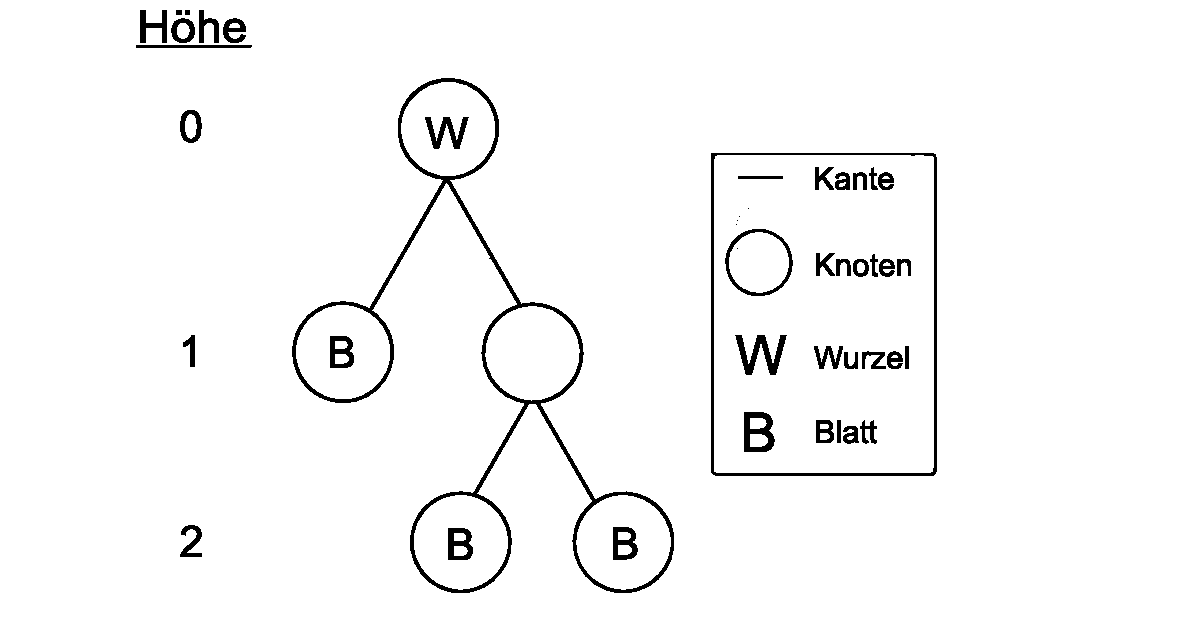
\includegraphics[scale = 0.5]{abbildungen/simple_tree}
    \caption{Einfacher beschrifteter Binärbaum}
    \label{pic:simple_tree} 
\end{figure}

Eine spezielle Form von Bäumen stellen die sogenannten Binärbäume dar. 
Binärbäume sind Bäume, wo jeder Knoten maximal zwei Kinder hat. Abbildung \ref{pic:simple_tree} 
zeigt einen einfachen Binärbaum, wo jedes Element genau beschriftet ist. 

Um jeden Knoten eines Baumes abarbeiten zu können, kann über dem Baum 
traversiert werden. Traversierung bezeichnet das systematische Ablaufen 
von jedem Knoten eines Baumes. Der naive Algorithmus
von Wetherell und Shannon verwendet die sogenannte
Pre-Order-Traversierung. Dabei wird zunächst der Knoten, dann der linke Teilbaum
und zum Schluss der rechte Teilbaum besucht. Hier werden die Väter also vor den
Kindern durchlaufen. Sowohl der verbesserte Algorithmus von Wetherell 
und Shannon als auch der Algorithmus von Reingold und Tilford verwenden hingegen die 
Post-Order-Traversierung. Dabei wird als erstes der linke Teilbaum, dann der 
rechte Teilbaum und dann der Knoten besucht \cite[]{q4}. Bei dieser Art der 
Traversierung werden die Kinder also vor den Väter durchlaufen. Neben diesen Arten
der Traversierung gibt es noch weitere Möglichkeiten, wie über einem 
Baum traversiert werden kann. Diese sind für das Verständnis der hier 
vorgestellten Algorithmen aber nicht notwendig.


\section{Anwendungsgebiete}

Bäume erfahren einen vielfältigen Einsatz in der Informatik, zum Beispiel 
als Datenstruktur, als Syntaxbäume, als Ausdrucksbäume oder auch als 
Entscheidungsbäume.

Ein Baum als Datenstruktur kann beispielsweise dazu verwendet werden, 
um eine Menge von Daten zu sortieren oder in ihnen effizient nach einen 
bestimmten Datensatz zu suchen. So verwendet der Heap-Sort-Algorithmus 
einen Baum zum Sortieren von Daten. Ebenso können Bäume dazu verwendet 
werden, die Syntax von Quellcode zu überprüfen. Ferner werden diese Bäume 
als Syntaxbäume bezeichnet. Zudem werden Bäume verwendet um mathematische 
Ausdrücke auszuwerten. Hierfür wird ein sogenannter Ausdrucksbaum für einen 
gegebenen mathematischen Ausdruck aufgestellt und ausgewertet. In der 
Datenanalyse werden Bäume in Form von Entscheidungsbäumen verwendet. 
Diese werden benutzt um Abhängigkeiten darzustellen. Die Blätter stellen 
Kategorien dar und die Knoten Bedingungen. So können beispielsweise neue 
Datensätze, in Abhängigkeit zu seinen Werten, einer bestimmten Kategorie 
zugeordnet werden.

Auch außerhalb der Informatik werden Bäume häufig verwendet. Sie können 
dazu verwendet werden um zum Beispiel eine Hierarchie eines Unternehmens 
(siehe Abb. 1) dazustellen oder einen Stammbaum einer 
Familie (siehe Abb. 2) \cite[]{q4}.

\todo{Zwei beispielhafte Abbildungen erstellen}
